\documentclass[12pt]{article}
\usepackage[utf8]{inputenc}
\usepackage[T1]{fontenc}
\usepackage[spanish]{babel}
\usepackage{indentfirst}
\usepackage{booktabs}
\usepackage{amsmath}
\usepackage{amsfonts}
\usepackage{graphicx}
\usepackage{float}
\usepackage{geometry}
\usepackage{hyperref}

\geometry{letterpaper, margin=2.5cm}
\graphicspath{{figures/}}
\hypersetup{
    colorlinks=true,
    linkcolor=blue,
    urlcolor=blue
}

\title{Informe de Simulación de Eventos Discretos\\Puerto Sobrecargado}
\author{Alberto E. Marichal Fonseca\\Grupo CD 311 \\ \url{https://github.com/ALbertE03/Discrete-event-simulation} }
\date{Mayo de 2026}

\begin{document}

\maketitle

\section{Orden del Problema Asignado}

El problema asignado es \textbf{Puerto Sobrecargado}. Se debe simular el funcionamiento de un puerto de supertanqueros con 3 muelles y un remolcador, con el objetivo de estimar los tiempos promedio de espera y analizar el comportamiento del sistema bajo las reglas de operación indicadas.

En el puerto llegan tanqueros de tres tamaños: pequeños, medianos y grandes. Todos necesitan asistencia del remolcador para entrar al muelle y para abandonar el puerto luego de terminar la carga. Los muelles son recursos limitados y el remolcador es un recurso único.

\begin{table}[H]
\centering
\caption{Parámetros de los tanqueros}
\begin{tabular}{lccc}
\toprule
\textbf{Tamaño} & \textbf{Pequeño} & \textbf{Mediano} & \textbf{Grande} \\
\midrule
Probabilidad de arribo & 0.25 & 0.25 & 0.50 \\
Tiempo de carga & $\mathcal{N}(9, 1)$ & $\mathcal{N}(12, 2)$ & $\mathcal{N}(18, 3)$ \\
\bottomrule
\end{tabular}
\end{table}


La solución se desarrolló como una simulación de eventos discretos. En lugar de avanzar el reloj en intervalos fijos, el modelo salta de un cambio relevante al siguiente: la llegada de un tanquero, el inicio o fin de un remolque, el comienzo o final de la carga y la salida del sistema. Para mantener ese orden temporal se utilizó una cola de prioridad con la lista de eventos futuros.

La operación del puerto se representó con dos colas FIFO: una para los barcos que esperan entrar desde el puerto y otra para los que ya terminaron de cargar y esperan salir desde los muelles. Los tres muelles se manejan como una capacidad limitada, mientras que el remolcador se trata como un recurso único que puede estar en el puerto, en la zona de muelles o viajando vacío entre ambas zonas. Cuando un barco inicia el remolque de entrada, el modelo reserva inmediatamente un muelle para evitar asignaciones duplicadas. Con esta lógica se ejecutaron 50 réplicas independientes de 100000 barcos cada una, suficientes para estimar promedios e intervalos de confianza.

\section{Modelo}

\subsection{Entidades}

El modelo se organiza alrededor de tres estructuras principales. \texttt{Ship} representa a cada tanquero y concentra su información operativa: tipo de barco, hora de llegada, duración de carga, momentos de remolque, inicio y fin de carga, inicio de salida y abandono del sistema. \texttt{Event} describe cada cambio futuro mediante su tiempo de ocurrencia, su tipo y, cuando aplica, el identificador del barco asociado. Sobre esas dos estructuras trabaja \texttt{PortSimulation}, que controla el reloj de simulación, administra la lista de eventos, actualiza las colas y recursos, y acumula las métricas finales.

\subsection{Eventos}

La dinámica del sistema comienza con la llegada de un nuevo tanquero. Si el barco puede entrar, se programa el fin del remolque de entrada y, al completarse ese traslado, empieza la carga. Cuando la carga termina, el barco pasa a la cola de salida. El ciclo se cierra cuando concluye el remolque de salida: el tanquero abandona el sistema, el muelle queda libre y puede atenderse otro barco.

También se modelan los desplazamientos vacíos del remolcador entre el puerto y la zona de muelles. Estos movimientos son importantes porque el remolcador no puede atender de inmediato una cola que se encuentra en la zona opuesta; primero debe completar el viaje vacío y recién entonces puede iniciar un nuevo remolque.

\subsection{Reglas del Remolcador}

Cuando el remolcador está en el puerto, primero intenta llevar al muelle al primer barco de la cola de entrada, siempre que exista al menos un muelle disponible. Si no puede entrar ningún barco y hay barcos esperando salir, viaja vacío hacia los muelles.

Cuando el remolcador está en los muelles, primero atiende a los barcos que esperan salir. Si no hay barcos esperando salir y hay barcos esperando entrar con algún muelle disponible, viaja vacío hacia el puerto.


\begin{table}[H]
\centering
\caption{Parámetros usados en la simulación}
\begin{tabular}{lc}
\toprule
\textbf{Proceso} & \textbf{Parámetro usado en \texttt{expovariate(L)}} \\
\midrule
Tiempo entre arribos & $\lambda = 8.0$ \\
Remolque de entrada & $\lambda = 2.0$ \\
Remolque de salida & $\lambda = 1.0$ \\
Viaje vacío del remolcador & $\lambda = 0.25$ \\
\bottomrule
\end{tabular}
\end{table}

Para los tiempos de carga se usaron distribuciones normales según el tipo de barco. Si una normal generaba un valor menor o igual que cero, se rechazaba y se volvía a muestrear.

\subsection{Métricas Calculadas}

Para cada barco completado se midió cuánto tarda en ser atendido desde que llega al puerto, cuánto demora en comenzar la carga, cuánto espera en el muelle después de cargar y cuánto tiempo permanece en total dentro del sistema. En términos de las variables registradas por la simulación, estas métricas corresponden a \texttt{inbound\_tow\_start - arrival\_time}, \texttt{loading\_start - arrival\_time}, \texttt{outbound\_tow\_start - loading\_end} y \texttt{departure\_time - arrival\_time}, respectivamente.

Los intervalos de confianza al 95\% se calcularon mediante:

\[
IC_{95\%} = \bar{x} \pm 1.96 \cdot \frac{s}{\sqrt{n}},
\]

donde $n=50$ réplicas.

\section{Resultados}

La configuración base simulada fue la del problema original: 3 muelles, 1 remolcador, 100000 barcos por réplica y 50 réplicas independientes. 

\begin{table}[H]
\centering
\caption{Resultados de la configuración base}
\label{tab:resultados-base}
\resizebox{\textwidth}{!}{%
\begin{tabular}{lrrrr}
\toprule
\textbf{Métrica} & \textbf{Media (h)} & \textbf{IC 95\% (h)} & \textbf{Mín. (h)} & \textbf{Máx. (h)} \\
\midrule
Espera antes del remolque de entrada & 260314.31 & $\pm$ 66.05 & 259764.87 & 261018.66 \\
Tiempo hasta comenzar carga & 260314.81 & $\pm$ 66.05 & 259765.37 & 261019.17 \\
Espera en muelle para salir & 0.2403 & $\pm$ 0.0007 & 0.2333 & 0.2456 \\
Tiempo total en el sistema & 260330.31 & $\pm$ 66.06 & 259780.83 & 261034.69 \\
\bottomrule
\end{tabular}
}
\end{table}

El tiempo promedio de espera en muelle para salir fue de $0.2403$ horas, equivalente aproximadamente a $14.42$ minutos. Sin embargo, la espera antes de iniciar el remolque de entrada fue extremadamente alta: $260314.31$ horas en promedio. Esto confirma que la congestión principal aparece antes de que los barcos logren entrar al muelle.

\begin{figure}[H]
\centering
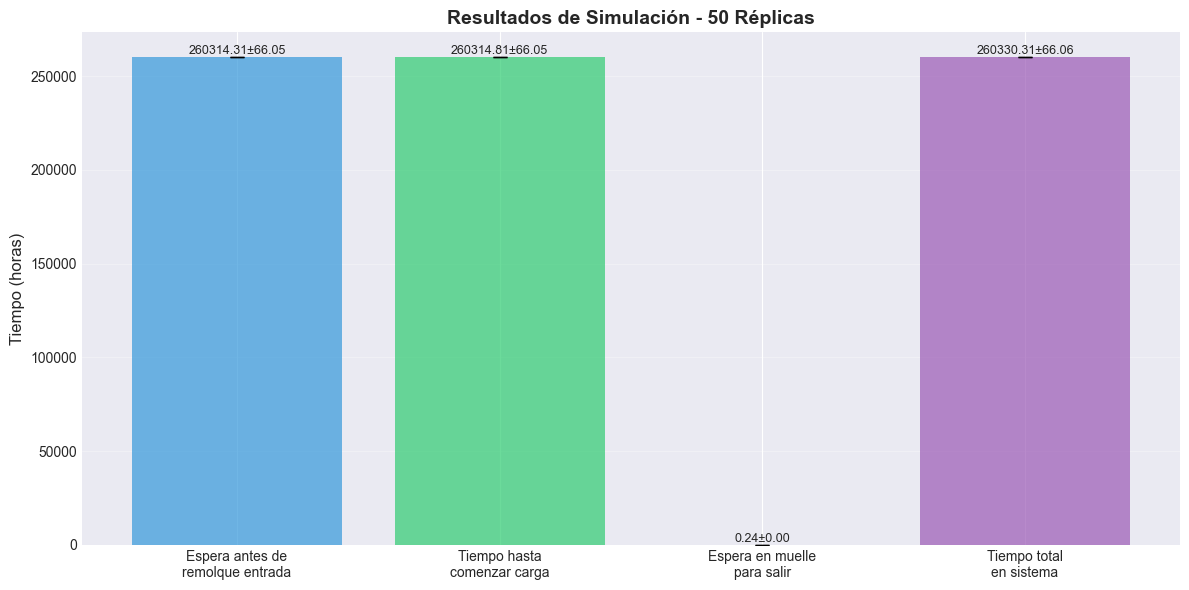
\includegraphics[width=0.95\textwidth]{resultados_metricas.png}
\caption{Promedios e intervalos de confianza de las métricas principales.}
\end{figure}

\begin{figure}[H]
\centering
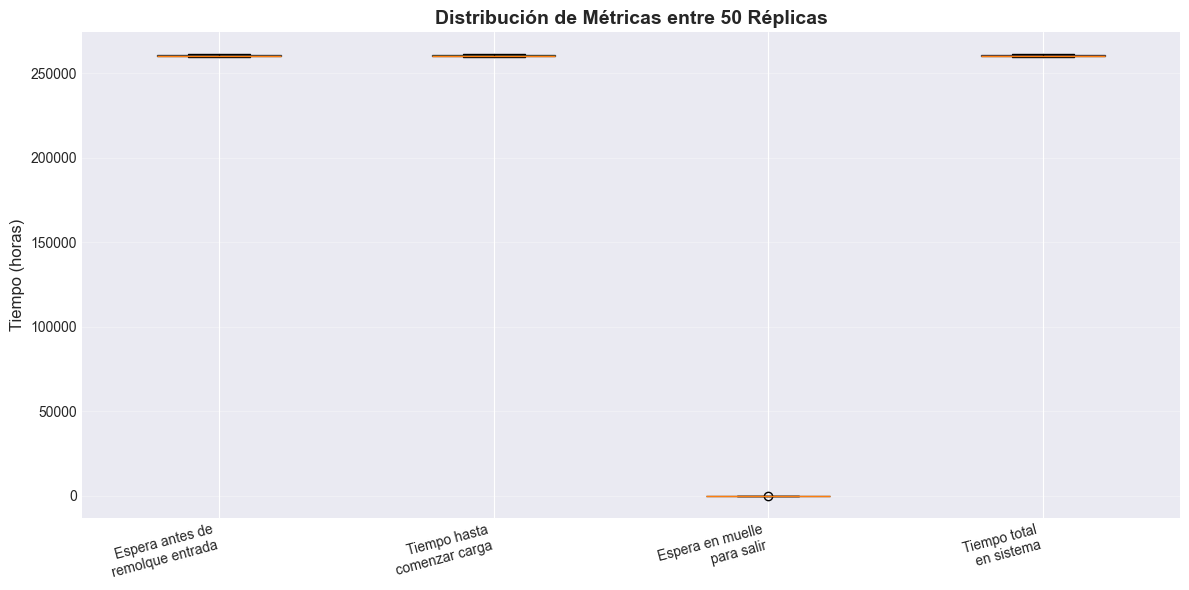
\includegraphics[width=0.95\textwidth]{distribucion_metricas.png}
\caption{Distribución de las métricas entre las 50 réplicas.}
\end{figure}

\begin{figure}[H]
\centering
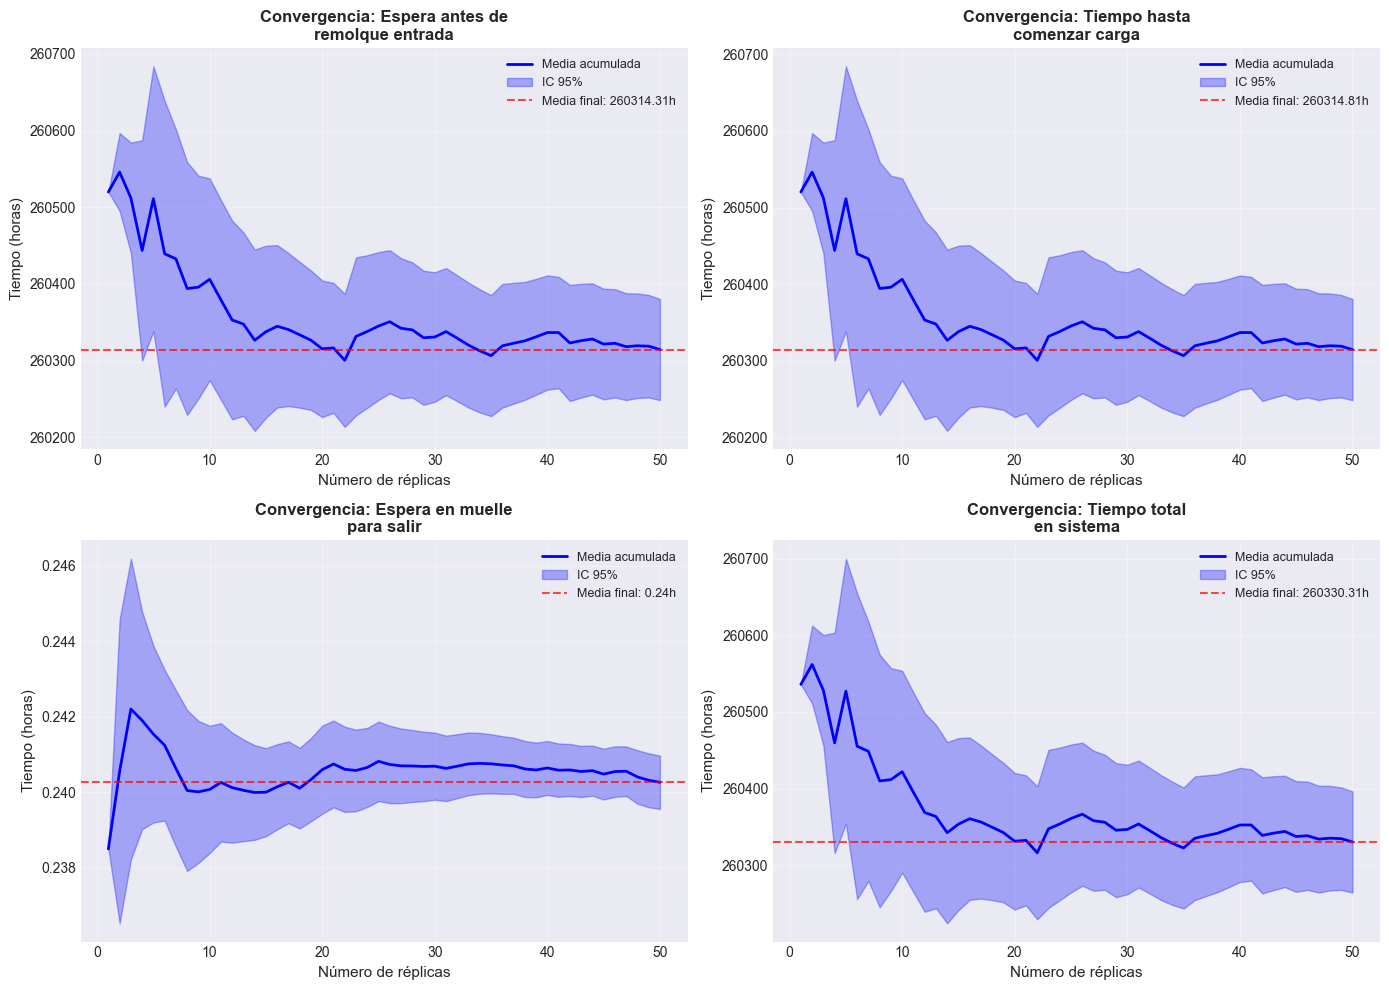
\includegraphics[width=0.95\textwidth]{convergencia_metricas.png}
\caption{Convergencia de las medias acumuladas y sus intervalos de confianza.}
\end{figure}

\begin{figure}[H]
\centering
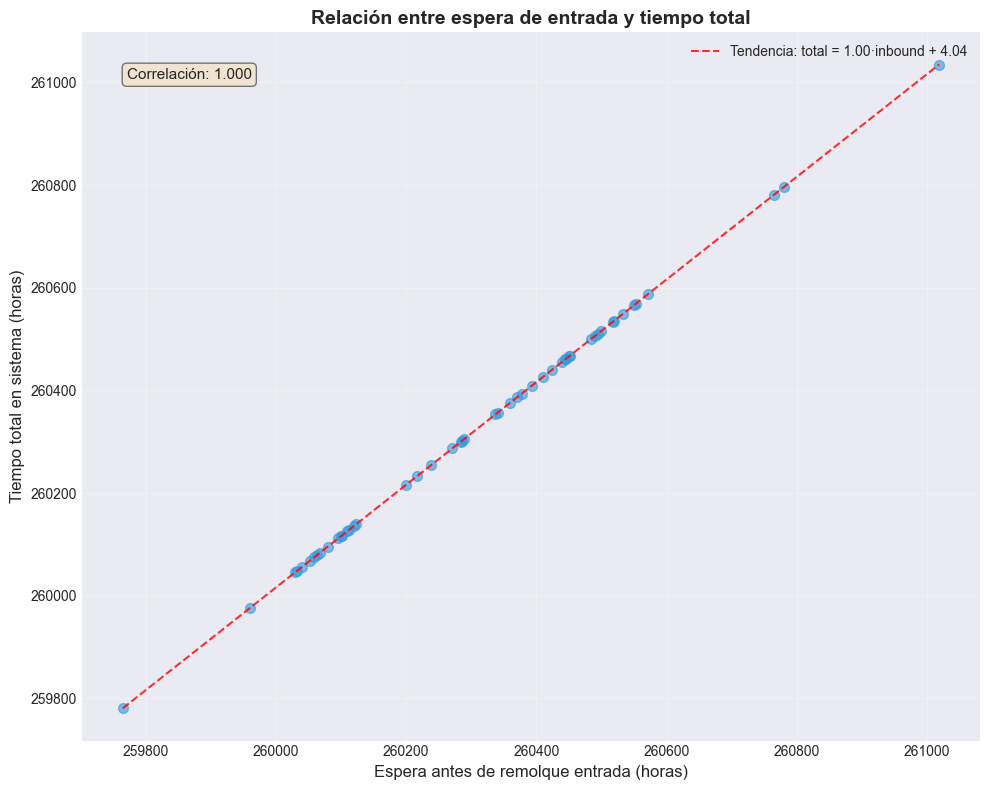
\includegraphics[width=0.82\textwidth]{relacion_espera_total.png}
\caption{Relación entre la espera de entrada y el tiempo total en el sistema.}
\end{figure}

\section{Experimentos con Más Muelles y Remolcadores}

Además de la configuración original, se ejecutó un análisis de sensibilidad con diferentes cantidades de muelles y remolcadores. El objetivo de estos experimentos fue observar qué tanto cambia la congestión al aumentar la capacidad del puerto.

Este análisis de sensibilidad usa un esquema de semillas diferente al de la corrida base detallada, por eso la fila \texttt{base\_3\_1} presenta pequeñas variaciones numéricas. La magnitud y la interpretación del comportamiento se mantienen.

\begin{table}[H]
\centering
\caption{Configuraciones evaluadas en el análisis de sensibilidad}
\label{tab:configuraciones}
\resizebox{\textwidth}{!}{%
\begin{tabular}{lcc}
\toprule
\textbf{Identificador} & \textbf{Muelles} & \textbf{Remolcadores} \\
\midrule
\texttt{base\_3\_1} & 3 & 1 \\
\texttt{mas\_remolcadores\_3\_2}  & 3 & 2 \\
\texttt{iguales\_3\_3} & 3 & 3 \\
\texttt{mas\_muelles\_4\_1} & 4 & 1 \\
\texttt{mejorado\_4\_2} & 4 & 2 \\
\texttt{extremo\_5\_1} & 5 & 1 \\
\texttt{extremo\_100\_1} & 100 & 1 \\
\texttt{extremo\_100\_50} & 100 & 50 \\
\texttt{extremo\_100\_70} & 100 & 70 \\
\bottomrule
\end{tabular}
}
\end{table}

\begin{table}[H]
\centering
\caption{Resumen de los experimentos de sensibilidad}
\label{tab:sensibilidad}
\resizebox{\textwidth}{!}{%
\begin{tabular}{lccccc}
\toprule
\textbf{Configuración} & \textbf{Muelles} & \textbf{Remolc.} & \textbf{Espera entrada (h)} & \textbf{Tiempo total (h)} & \textbf{Mejora} \\
\midrule
\texttt{base\_3\_1} & 3 & 1 & $260264.61 \pm 82.95$ & $260280.60 \pm 82.96$ & $+0.0\%$ \\
\texttt{mas\_remolcadores\_3\_2} & 3 & 2 & $260259.03 \pm 66.28$ & $260275.02 \pm 66.28$ & $+0.0\%$ \\
\texttt{iguales\_3\_3} & 3 & 3 & $260201.43 \pm 67.11$ & $260217.41 \pm 67.11$ & $+0.0\%$ \\
\texttt{mas\_muelles\_4\_1} & 4 & 1 & $195564.29 \pm 55.51$ & $195580.44 \pm 55.51$ & $+24.9\%$ \\
\texttt{mejorado\_4\_2} & 4 & 2 & $195540.41 \pm 58.42$ & $195556.55 \pm 58.42$ & $+24.9\%$ \\
\texttt{extremo\_5\_1} & 5 & 1 & $157023.57 \pm 48.94$ & $157039.90 \pm 48.94$ & $+39.7\%$ \\
\texttt{extremo\_100\_1} & 100 & 1 & $68821.57 \pm 58.34$ & $68854.25 \pm 58.34$ & $+73.6\%$ \\
\texttt{extremo\_100\_50} & 100 & 50 & $68797.93 \pm 51.02$ & $68830.61 \pm 51.02$ & $+73.6\%$ \\
\texttt{extremo\_100\_70} & 100 & 70 & $68830.43 \pm 55.53$ & $68863.13 \pm 55.58$ & $+73.6\%$ \\
\bottomrule
\end{tabular}
}
\end{table}

\begin{figure}[H]
\centering
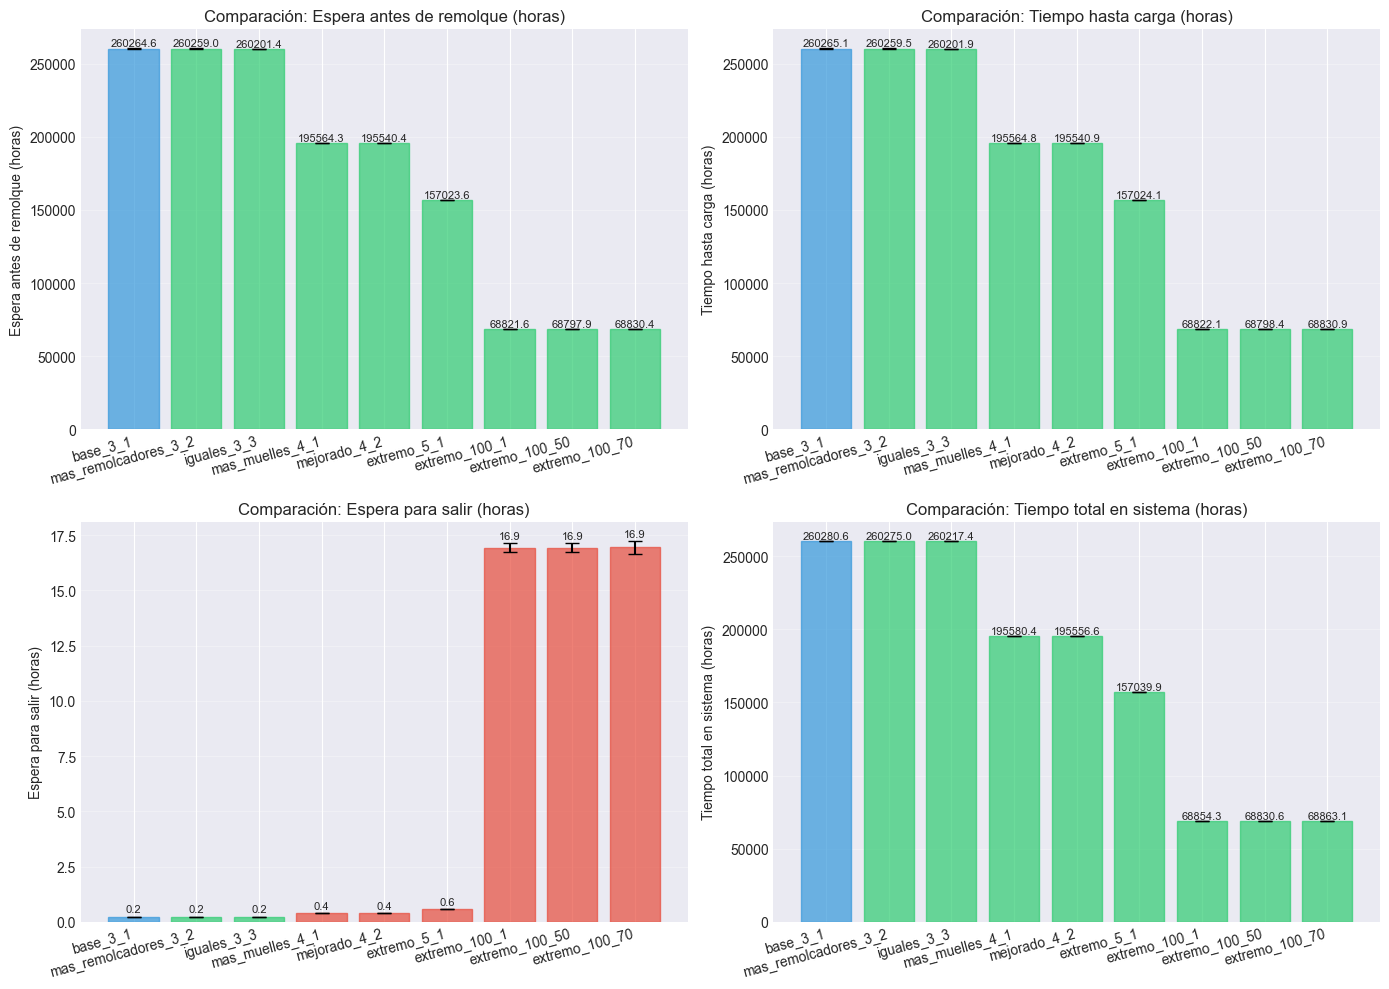
\includegraphics[width=0.95\textwidth]{sensibilidad_comparacion.png}
\caption{Comparación de las métricas principales entre configuraciones.}
\end{figure}

\begin{figure}[H]
\centering
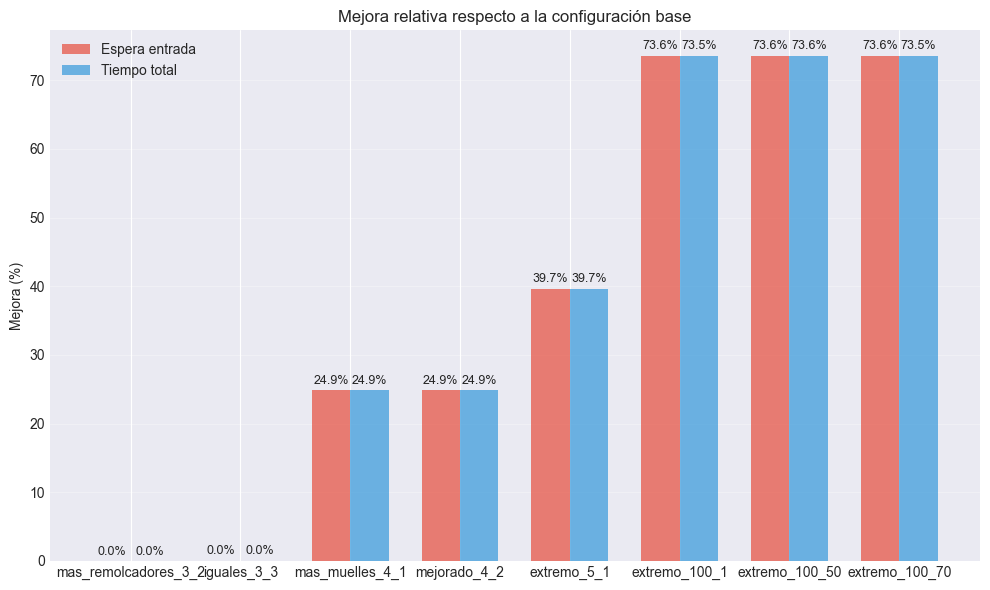
\includegraphics[width=0.90\textwidth]{sensibilidad_mejora_relativa.png}
\caption{Mejora relativa respecto a la configuración base.}
\end{figure}

El análisis ANOVA reportado dio diferencias significativas entre configuraciones para la espera de entrada y para el tiempo total en sistema, con $p < 0.05$ en ambos casos. Las comparaciones por pares muestran que aumentar de 3 a 4 muelles, de 4 a 5 muelles y luego hasta 100 muelles reduce de forma significativa la espera de entrada. En cambio, para un mismo número de muelles, aumentar solamente la cantidad de remolcadores no produjo diferencias significativas en las salidas obtenidas.

Los experimentos más interesantes fueron los de aumento de muelles. Pasar de 3 a 4 muelles redujo la espera de entrada en aproximadamente $24.9\%$, mientras que usar 5 muelles alcanzó una mejora cercana al $39.7\%$. Los escenarios extremos con 100 muelles redujeron la espera de entrada en aproximadamente $73.6\%$, aunque el sistema siguió mostrando tiempos de espera elevados por la intensidad de los arribos.

\section{Consideraciones Obtenidas a Partir de las Simulaciones}

El comportamiento observado corresponde a un sistema claramente sobrecargado. Con el uso directo de \texttt{expovariate($\lambda$)} y $\lambda=8$ para los arribos, los tanqueros se incorporan al puerto a un ritmo muy superior al que la infraestructura puede absorber. La limitación no proviene de un solo elemento aislado: los tres muelles, el remolcador único y los tiempos de carga actúan en conjunto, especialmente porque la mitad de los barcos son grandes y permanecen más tiempo ocupando capacidad.

La espera antes del remolque de entrada domina casi por completo el tiempo total en el sistema. La diferencia entre esperar el remolque y comenzar la carga es pequeña, de modo que el traslado de entrada no explica la congestión principal una vez que el barco logra ser atendido. El problema aparece antes, cuando la cola de entrada crece porque no hay suficiente capacidad disponible para iniciar nuevas cargas.

Después de la carga, el panorama es distinto. La espera para salir desde el muelle fue baja en comparación con la espera de entrada, lo cual indica que los barcos no quedan demasiado tiempo retenidos al finalizar su servicio. Aun así, esa eficiencia local no compensa la acumulación inicial: el sistema sigue siendo inestable dentro del horizonte simulado porque la demanda supera la capacidad efectiva del puerto.

El análisis de sensibilidad refuerza esta lectura. Agregar remolcadores, sin aumentar el número de muelles, produjo cambios muy pequeños; en cambio, ampliar los muelles redujo la espera de forma visible. Por eso, una mejora real tendría que actuar sobre la capacidad de entrada y carga del puerto, o sobre la frecuencia de arribos, antes que concentrarse solamente en acelerar la salida desde los muelles.

\section{Conclusiones}

La simulación confirma que el puerto opera en una condición de sobrecarga. Aunque la espera promedio para salir del muelle fue baja, $0.2403$ horas o aproximadamente $14.42$ minutos, la espera antes de comenzar el proceso de entrada alcanzó $260314.31$ horas. Como consecuencia, el tiempo total promedio en el sistema, $260330.31$ horas, queda determinado casi por completo por esa acumulación inicial.

Los experimentos de sensibilidad muestran que el cambio con mayor efecto fue aumentar la cantidad de muelles. Pasar de 3 a 4 muelles redujo la espera de entrada en $24.9\%$, y usar 5 muelles elevó la mejora a $39.7\%$. Incluso los escenarios extremos con 100 muelles, que alcanzaron una reducción cercana al $73.6\%$, no eliminaron por completo la congestión, lo cual confirma que la intensidad de los arribos mantiene al sistema bajo presión.

El ANOVA también respalda esta interpretación: existen diferencias significativas entre configuraciones, pero las variaciones relevantes se asocian principalmente al aumento de muelles. En síntesis, el principal problema operativo no está en la salida de los barcos ya cargados, sino en la capacidad del puerto para admitir nuevos tanqueros y sostener el ritmo de carga frente a la demanda simulada.

\end{document}
